\documentclass[xcolor=dvipsnames]{beamer}
\title{Realtime Embedded Coding: drivers / callback}
\date{}
\author{Bernd Porr}
\begin{document}
\begin{frame}
\titlepage
\end{frame}

\begin{frame}[fragile]
\frametitle{Callbacks}
\begin{figure}[!hbt]
    \begin{center}
    \mbox{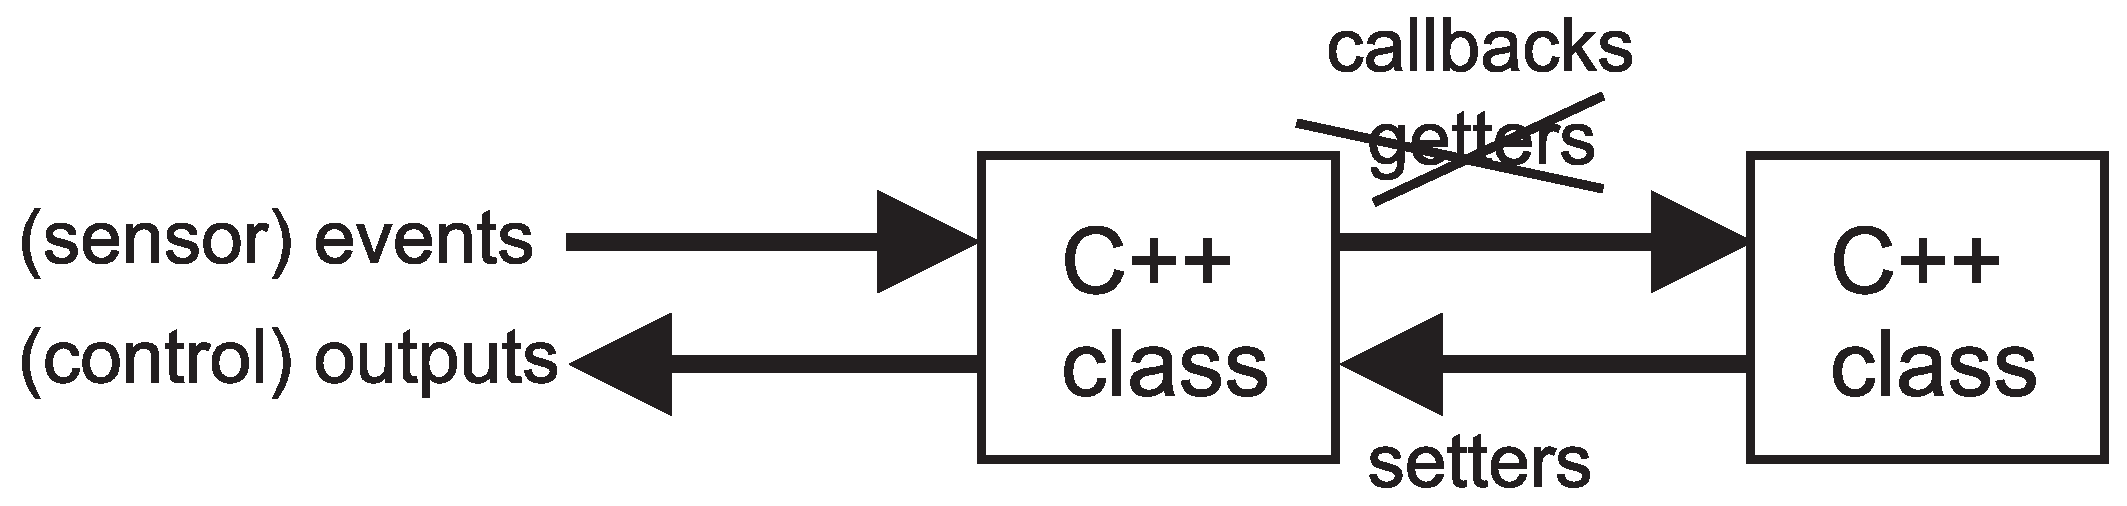
\includegraphics[width=\textwidth]{gettersetters}}
    \end{center}
    A realtime system with two C++ classes. Communication
      between classes is achieved with callbacks (not getters) for incoming events
      and setters to send out control events. The control output itself
      receives its timing from the events so that the loop is traversed
      as quickly as possible.
    \end{figure}
\end{frame}


\begin{frame}[fragile]
    \frametitle{SOLID}

\textbf{Open-Closed principle:} Your class is open to extension but
closed to modification. 

\textbf{Liskov substitution principle:} Strictly, substituting
a derived class for its base class does not result in the program
becoming incorrect. 

\textbf{Interface Segregation principle:}
Keep functionality separate and aim to divide it up in different
classes. 

\textbf{Dependency inversion:} That is about abstracting the
essential features of a class of interfaces.

\end{frame}

\begin{frame}[fragile]
    \frametitle{Mandatory coding requirements}
    It's essential that:
\begin{enumerate}
\item you use \textbf{C++11 (or later) memory management}: copy constructors, standard template library (STL) containers and no raw pointers
  managed with new/delete.
\item the project has a \textbf{build system} such as \textbf{cmake}.
\item classes (in particular driver classes) are \textbf{re-usable}
  outwith of the specific project.
\item all public interfaces have \textbf{doc-strings} for all public
  methods/constants and an automatically generated reference, for
  example with the help of \textbf{doxygen}.
\item classes which perform internal processing such as filters,
  databases, detectors, \ldots, have \textbf{unit tests} and are run via
  the cmake testing framework.
\item the documentation provides comprehensive information about the project itself,
  how to install and run the project.
\end{enumerate}
\end{frame}
    
    

\begin{frame}[fragile]
    \frametitle{Device driver C++ classes}
\begin{enumerate}
    \item Setters and callbacks hand over \textsl{physical units}
      (temperature, acceleration, \ldots) or relative units but not raw
      integer values with no meaning.
    \item The sensor is configured by specifying physical units (time,
      voltage, temperature) and not sensor registers. Default config parameters
      should be specified that the class can be used straight away with
      default parameters.
    \item The class comes with simple demo programs demonstrating how
      a client program might use it.
    \end{enumerate}
\end{frame}
 

\begin{frame}[fragile]
    \frametitle{C++ callback interface}

Callback interface:
\begin{verbatim}
class LSM9DS1callback {
public:
        virtual void hasSample(LSM9DS1Sample sample) = 0;
};
\end{verbatim}

C++ driver class:
\begin{verbatim}
void LSM9DS1::dataReady() {
        LSM9DS1Sample sample;
        // fills the sample struct with data
        // ...
        lsm9ds1Callback->hasSample(sample);
}
\end{verbatim}

C++ driver callback registration:
\begin{verbatim}
void LSM9DS1::registerCallback(LSM9DS1callback* cb);
\end{verbatim}

\end{frame}



\begin{frame}[fragile]
    \frametitle{Merging C++ driver class and callback interface}
Instead of creating a separate class containing the callback you
can also add the callback straight to the device driver class.
\begin{verbatim}
class ADS1115rpi {
        ...
        virtual void hasSample(float sample) = 0;
        ...
};
\end{verbatim}
This forces the client to implement the callback to be able to use
the class. This creates a very safe environment as all dependencies
are set at compile time and the abstract nature of the base class
makes clear what needs to be implemented.
See
\url{https://github.com/berndporr/rpi_ads1115} for a complete example.
\end{frame}



\begin{frame}[fragile]
    \frametitle{Callback arguments}
Often more than one sample or more complex data are transmitted:
Complex data: do not put loads of arguments into the
  callback but define a \textsl{struct}. For example an ADC might
  deliver all 4 channels at once:
\begin{verbatim}
class ADmulti {

        struct ADCSample {
            float ch1;
            float ch2;
            float ch3;
            float ch4;
        };

        ...
        virtual void hasSample(ADCSample& sample) = 0;
        ...
};
\end{verbatim}
\end{frame}



\begin{frame}[fragile]
    \frametitle{GPIO events}

    \begin{verbatim}
class mySensorClass {
    static void gpioISR(int g, int l, uint32_t, void* usr)
    ...
}
        \end{verbatim}
        is registered with pigpio:
        \begin{verbatim}
gpioSetISRFuncEx(24,RISING_EDGE,ISR_TIMEOUT,gpioISR,
                 (void*)this);
        \end{verbatim}
        The callback registered will then be \texttt{this->dataReady()}.
        \begin{verbatim}
class LSM9DS1 {
    void dataReady();
    static void gpioISR(int gpio, int level, uint32_t tick, void* userdata)
    {
        ((LSM9DS1*)userdata)->dataReady();
    }
};
        \end{verbatim}

    \end{frame}




    \begin{frame}[fragile]
\frametitle{Video camera capture (openCV)}
Reading from a video camera is usually done with the help of openCV
which is a wrapper around the raw video 4 Linux devices. These are
blocking to establish the capture events so that a loop needs to run in
a thread:
\begin{verbatim}
while(running) {
    cv::Mat cap;
    videoCapture.read(cap);   // <---- BLOCKING! :)
    sceneCallback->nextScene(cap);
}
\end{verbatim}
The \texttt{read(cap)} command is blocking till a new frame has
arrived which is then transmitted with the callback \texttt{nextScene}
to the client. The full code of the example camera class is here:
\url{https://github.com/berndporr/opencv-camera-callback}.
\end{frame}


\begin{frame}[fragile]
    \frametitle{Recording audio}
\begin{verbatim}
    while (running) {
      if ((err = snd_pcm_readi (handle, buffer, buffer_frames)) != buffer_frames) {
        if (errCallback) errCallback->hasError();
      }
      if (sampleCallback) sampleCallback->hasData(buffer);
    }
   \end{verbatim}
\end{frame}



\begin{frame}[fragile]
    \frametitle{I2C}
\begin{verbatim}
int fd = i2cOpen(i2c_bus, address, 0);
i2cWriteByteData(fd, subAddress, data);
i2cClose(fd);
\end{verbatim}
where \texttt{i2c\_bus} is the I2C bus number (usually 1 on the RPI)
and the \texttt{address} is the I2C address of the device on that bus.
The \texttt{subAddress} here is the register address in the device.


\textbf{Important}: I2C (and SPI) is blocking but only for duration of the transmission or reception!
Usually it won't wait for an event. Use GPIO for the events (data-ready).
\end{frame}

\begin{frame}[fragile]
    \frametitle{Summary}

    \begin{itemize}
        \item Events are transmitted via callback interfaces between classes by using abstract virtual methods.
        \item Events are generated by blocking I/O.
    \end{itemize}
\end{frame}

\end{document}